% ============================================================
%  main.tex  –  Heart Disease Detection Research Proposal
%  Compile order:  pdflatex -> bibtex -> pdflatex -> pdflatex
% ============================================================
\documentclass[12pt, a4paper]{article}

% -- Layout ---------------------------------------------------
\usepackage[a4paper, top=2.5cm, bottom=2.5cm,
            left=3cm, right=2.5cm]{geometry}
\setlength{\parskip}{6pt}
\setlength{\headheight}{15pt}
\setlength{\parindent}{0pt}

% -- Typography & encoding ------------------------------------
\usepackage[T1]{fontenc}
\usepackage[utf8]{inputenc}
\usepackage[protrusion=true,expansion=false]{microtype}

% -- Maths ----------------------------------------------------
\usepackage{amsmath}
\usepackage{amssymb}

% -- Tables & figures -----------------------------------------
\usepackage{graphicx}
\usepackage{float}
\usepackage{booktabs}
\usepackage{longtable}
\usepackage{array}
\usepackage{tabularx}
\usepackage{ragged2e}
\usepackage{colortbl}

% -- Color & decoration ---------------------------------------
\usepackage{xcolor}
\usepackage{tikz}
\usepackage{pgffor}
\usetikzlibrary{calc}
\usepackage{mdframed}

% -- URLs -----------------------------------------------------
\usepackage{url}

% -- Header / Footer ------------------------------------------
\usepackage{fancyhdr}

% -- Bibliography ---------------------------------------------
\usepackage[numbers, sort&compress]{natbib}

% -- Navigable PDF  (load LAST) -------------------------------
\usepackage[
  colorlinks  = true,
  linkcolor   = black,
  citecolor   = blue,
  urlcolor    = blue,
  bookmarks   = true,
  bookmarksnumbered = true,
  pdftitle    = {Early Detection of Heart Disease Using Machine Learning},
  pdfauthor   = {Sadat Amir},
  pdfsubject  = {CS Research Proposal},
  pdfkeywords = {heart disease; machine learning; SVM; random forest}
]{hyperref}
\usepackage{hypernat}

% -- Define brand colours -------------------------------------
\definecolor{darknavy}{HTML}{0D1B2A}
\definecolor{mednavy}{HTML}{1B3A5C}
\definecolor{accent}{HTML}{E63946}
\definecolor{gold}{HTML}{F4A261}
\definecolor{lightgray}{HTML}{F5F5F5}
\definecolor{midgray}{HTML}{CCCCCC}

% -- Running-head style ---------------------------------------
\pagestyle{fancy}
\fancyhf{}
\renewcommand{\headrulewidth}{0.6pt}
\renewcommand{\headrule}{%
  {\color{mednavy}\hrule width\headwidth height 0.6pt}}
\fancyhead[L]{%
  \small\color{mednavy}\textbf{Early Detection of Heart Disease Using Machine Learning}}
\fancyhead[R]{\small\color{mednavy}Sadat Amir}
\fancyfoot[C]{\small\color{midgray}\thepage}

% plain style for first page of each section
\fancypagestyle{plain}{%
  \fancyhf{}
  \renewcommand{\headrulewidth}{0pt}
  \fancyfoot[C]{\small\color{midgray}\thepage}}

% -----------------------------------------------------------
\begin{document}

% ===========================================================
%  COVER PAGE
% ===========================================================
\begin{titlepage}
\thispagestyle{empty}
\pagecolor{darknavy}

\begin{tikzpicture}[remember picture, overlay]
  \fill[mednavy!70]
    (current page.north east)
    -- ++(-7cm, 0)
    -- ++(0, -4cm)
    -- ++(7cm, 0)
    -- cycle;
  \fill[accent]
    (current page.north west) ++(0,-4.35cm)
    rectangle ++(21cm, 0.18cm);
  \fill[accent]
    (current page.south west)
    rectangle ++(21cm, 0.6cm);
  \foreach \r/\op in {3.5cm/0.08, 2.5cm/0.12, 1.5cm/0.18}{
    \fill[white, opacity=\op]
      (current page.south east) ++(-1.5cm, 1.5cm) circle (\r);
  }
  \fill[gold, opacity=0.25]
    (current page.north west) ++(0.8cm,-0.8cm)
    rectangle ++(2.5cm,-2.5cm);
  \fill[gold, opacity=0.45]
    (current page.north west) ++(1cm,-1cm)
    rectangle ++(1.5cm,-1.5cm);
\end{tikzpicture}

\vspace*{1.0cm}

\begin{center}
  {\fontsize{22}{26}\selectfont\bfseries\color{white}%
    HAWASSA UNIVERSITY}\\[0.25cm]
  {\small\color{midgray}\textit{Institute of Technology
    \textbullet\ Computer Science Department}}\\[0.2cm]
  {\footnotesize\color{gold}%
    Course: Research Methods in Computer Science (CoSc3101)}
\end{center}

\vspace{0.6cm}
{\color{accent}\hrule height 1.6pt}\vspace{2pt}
{\color{gold!60}\hrule height 0.5pt}

\vspace{1.0cm}

\begin{center}
  {\fontsize{20}{26}\selectfont\bfseries\color{white}%
    Early Detection of Heart Disease\\[0.3cm]
    Using Machine Learning Techniques\\[0.3cm]
    on Patient Health Data}
\end{center}

\vspace{0.9cm}
{\color{gold!60}\hrule height 0.5pt}\vspace{2pt}
{\color{accent}\hrule height 1.6pt}

\vspace{1.6cm}

\begin{center}
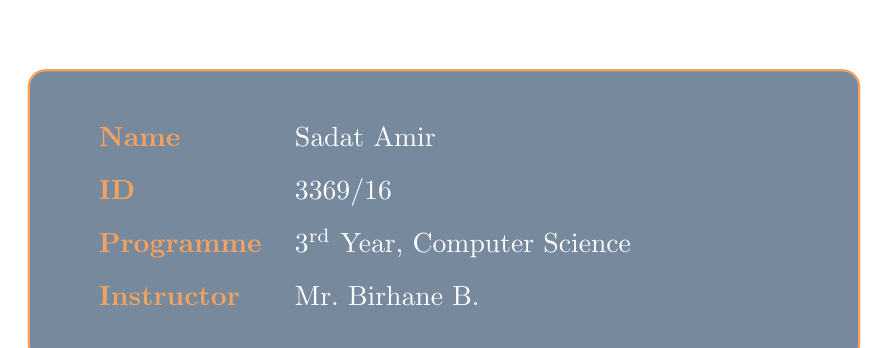
\begin{tikzpicture}
  \node[
    draw=gold, line width=0.8pt,
    rounded corners=6pt,
    fill=mednavy!60,
    inner xsep=22pt, inner ysep=14pt,
    text width=9cm
  ]{%
    \color{white}
    \renewcommand{\arraystretch}{1.6}
    \begin{tabular}{@{}ll@{}}
      \color{gold}\bfseries Name   & Sadat Amir \\
      \color{gold}\bfseries ID     & 3369/16 \\
      \color{gold}\bfseries Programme & 3\textsuperscript{rd} Year, Computer Science \\
      \color{gold}\bfseries Instructor & Mr.\ Birhane B. \\
   
    \end{tabular}
  };
\end{tikzpicture}
\end{center}
\color{white}\bfseries Repository: &
\href{https://github.com/s-a-d-a-t/Early-Detection-of-Heart-Disease-Using-Machine-Learning}
{\color{gold}My GitHub Repository} \\

\vfill

\begin{center}
  \foreach \kw in {Machine Learning, Heart Disease, SVM, Random Forest,
                   Logistic Regression, UCI Dataset}{%
    \tikz\node[
      fill=accent!80, rounded corners=3pt,
      inner xsep=6pt, inner ysep=3pt,
      font=\tiny\bfseries\color{white}
    ]{\kw};~%
  }
\end{center}

\vspace{0.5cm}

\end{titlepage}

\nopagecolor

% ===========================================================
%  TABLE OF CONTENTS
% ===========================================================
\tableofcontents
\newpage

% ===========================================================
%  ABSTRACT
% ===========================================================
\section*{Abstract}
\addcontentsline{toc}{section}{Abstract}

Early detection of heart disease is important for improving patient outcomes and
reducing healthcare costs, especially in low-resource settings. This study uses
machine learning techniques to detect heart disease at an early stage using
patient health data. Publicly available datasets, such as the combined Heart
Disease Dataset from the UCI Machine Learning Repository~\cite{uci_heart}, are
used for analysis. The data are preprocessed and used to train machine learning
models, including Random Forest, Logistic Regression, and Support Vector Machine
(SVM)~\cite{rf_heart2021}. Model performance is evaluated using
accuracy, precision, recall, F1-score, and ROC-AUC. The expected outcome is a
reliable, resource-efficient system that assists healthcare providers in making
faster and more accurate diagnostic decisions.


% ===========================================================
%  1. INTRODUCTION
% ===========================================================
\section{Introduction}

Heart disease is among the most serious global health challenges, accounting for
approximately 17.9 million deaths annually---about 32\% of all global deaths---
according to the World Health Organization (WHO)~\cite{who2023}. A critical
driver of this mortality rate is late diagnosis, particularly in low-resource
settings where traditional diagnostic methods are often too costly or
inaccessible. The limited availability of trained healthcare professionals and
the fact that many patients remain asymptomatic in early stages create
significant barriers to timely intervention. Machine learning offers a promising
solution by analysing patient health data to identify patterns that predict heart
disease early. By providing accessible, data-driven insights, this technology
can support healthcare providers in making faster, more accurate decisions to
improve patient outcomes.

\subsection{Problem Statement}

The problem is defined using the standard three-part structure
(Ideal $\rightarrow$ Reality $\rightarrow$ Consequence).

\textbf{Ideal:} In an ideal healthcare environment, cardiovascular health is monitored proactively through the systematic analysis of patient data---blood pressure, cholesterol, and medical history. Automated diagnostic systems would flag the early signs of heart disease even when patients are asymptomatic, allowing timely interventions that reduce mortality and make efficient use of healthcare resources.

\textbf{Reality:} Heart disease diagnosis is largely reactive, occurring only after a patient develops severe symptoms or suffers a cardiac event. While the WHO identifies cardiovascular disease as the leading cause of death globally~\cite{who2023}, many healthcare systems---especially in low-resource settings---lack the specialised professionals and expensive diagnostic tools needed for early screening.

\textbf{Consequence:} Heart disease often remains undetected until it is severe or irreversible, leading to high mortality rates and increased long-term costs. Without intelligent, data-driven tools, the gap between patient data and timely diagnosis will continue to grow, leaving millions of at-risk individuals without life-saving early intervention.

\subsection{Objectives}

The primary goal is to develop a reliable, accurate predictive model for the
early detection of heart disease using clinical data. By leveraging machine
learning, this study aims to provide healthcare providers with an accessible
tool for identifying cardiovascular risks early, enabling timely intervention
and significantly improving patient survival rates.

\subsubsection{General Objective}
To design and implement a machine learning-based framework that utilises patient
health data to accurately predict the early onset of heart disease, supporting
faster and more informed clinical decisions in both standard and resource-limited
healthcare settings.

\subsubsection{Specific Objectives}
The following SMART (Specific, Measurable, Achievable, Relevant, Time-bound)
objectives will be pursued:

\begin{enumerate}
  \item \textbf{Data Strategy and Preprocessing.} Collect structured heart
    disease data from the UCI Machine Learning Repository~\cite{uci_heart} and
    perform rigorous preprocessing---missing-value imputation, Min-Max
    normalisation, and feature encoding---to ensure data quality for model
    training.

  \item \textbf{Model Development and Training.} Develop and train at least
    three supervised machine learning models---Random Forest, Logistic
    Regression, and SVM~\cite{rf_heart2021}---to identify the
    most effective architecture for cardiac risk prediction.

  \item \textbf{Model Evaluation and Clinical Insight Generation.} Evaluate the trained models using accuracy, precision, recall, $F_1$-score, and ROC-AUC, targeting a minimum sensitivity (recall) of $0.90$ to minimize undiagnosed cases, while concurrently analyzing feature importance to identify significant health indicators for clinical decision support.
\end{enumerate}

% ===========================================================
%  2. LITERATURE SYNTHESIS & SOTA
% ===========================================================
\section{Literature Synthesis \& State of the Art}

% -----------------------------------------------------------
\subsection{Identification of Peer-Reviewed Sources}
% -----------------------------------------------------------

The five sources below were identified from IEEE Xplore, ACM Digital Library,
and Elsevier ScienceDirect (2022--2026). Each is described individually.

\medskip
\noindent\textbf{Source 1 --- Singh et al.\ \cite{singh2024} \hfill \textit{IEEE Xplore, 2024}}
\begin{itemize}
  \item \textbf{Method:} Compares Logistic Regression, SVM, KNN, and Random Forest
        for binary heart disease classification.
  \item \textbf{Dataset:} UCI Heart Disease benchmark (303 records).
  \item \textbf{Key result:} Best accuracy of 85.25\% achieved with Random Forest.
  \item \textbf{Limitation:} Small sample size restricts generalisation to broader
        or more diverse patient populations.
\end{itemize}

\medskip
\noindent\textbf{Source 2 --- Bhatt et al.\ \cite{bhatt2023} \hfill \textit{ScienceDirect, 2023}}
\begin{itemize}
  \item \textbf{Method:} Applies Multilayer Perceptron (MLP), Random Forest, and
        SVM to cardiac risk prediction.
  \item \textbf{Dataset:} UCI Cleveland cohort.
  \item \textbf{Key result:} MLP achieves a high accuracy of 98.22\%.
  \item \textbf{Limitation:} Deep MLP training demands significant compute resources,
        making it impractical on low-end clinic hardware.
\end{itemize}

\medskip
\noindent\textbf{Source 3 --- Chang et al.\ \cite{chang2022} \hfill \textit{IEEE Xplore, 2022}}
\begin{itemize}
  \item \textbf{Method:} Python-based pipeline using Random Forest, KNN, and
        Decision Tree classifiers.
  \item \textbf{Dataset:} Cleveland Heart Disease dataset.
  \item \textbf{Key result:} Random Forest reaches 96.0\% accuracy.
  \item \textbf{Limitation:} No clinician-facing user interface; limits practical
        deployment in real clinical environments.
\end{itemize}

\medskip
\noindent\textbf{Source 4 --- Pathan et al.\ \cite{pathan2022} \hfill \textit{ACM Digital Library, 2022}}
\begin{itemize}
  \item \textbf{Method:} Feature selection combined with SVM for optimised
        cardiac prediction.
  \item \textbf{Dataset:} Healthcare analytics dataset.
  \item \textbf{Key result:} Achieves an F1-score of 92.4\% after feature reduction.
  \item \textbf{Limitation:} Aggressive dimensionality reduction risks discarding
        subtle but clinically meaningful risk signals.
\end{itemize}

\medskip
\noindent\textbf{Source 5 --- Subahi et al.\ \cite{subahi2022} \hfill \textit{ScienceDirect, 2022}}
\begin{itemize}
  \item \textbf{Method:} Self-adaptive Bayesian classifier integrated with IoT
        wearable devices for continuous cardiac monitoring.
  \item \textbf{Dataset:} IoT-collected cardiac sensor data.
  \item \textbf{Key result:} Achieves 91.0\% precision in real-time risk detection.
  \item \textbf{Limitation:} Depends on stable IoT infrastructure, making it
        unreliable in rural or low-resource settings.
\end{itemize}

% -----------------------------------------------------------


% -----------------------------------------------------------
\subsection{Synthesis Matrix}
% -----------------------------------------------------------

Table~\ref{tab:synthesis} compares the five identified sources, summarising
their machine learning methods, datasets, reported performance metrics, and
key limitations.

\small
\renewcommand{\arraystretch}{1.35}

\begin{longtable}{@{}
  >{\RaggedRight\arraybackslash}p{2.4cm}
  >{\RaggedRight\arraybackslash}p{3.4cm}
  >{\RaggedRight\arraybackslash}p{2.4cm}
  >{\Centering\arraybackslash}p{1.9cm}
  >{\RaggedRight\arraybackslash}p{4.1cm}@{}}

\caption{Synthesis Matrix of Recent Research (2022--2026)}
\label{tab:synthesis}\\

\toprule
\rowcolor{darknavy}
\textcolor{white}{\textbf{Author \& Year}} &
\textcolor{white}{\textbf{Method}} &
\textcolor{white}{\textbf{Dataset}} &
\textcolor{white}{\textbf{Metric}} &
\textcolor{white}{\textbf{Limitation}}\\
\midrule
\endfirsthead

\multicolumn{5}{c}{\small\itshape (Table~\ref*{tab:synthesis} continued)}\\[2pt]
\toprule
\rowcolor{darknavy}
\textcolor{white}{\textbf{Author \& Year}} &
\textcolor{white}{\textbf{Method}} &
\textcolor{white}{\textbf{Dataset}} &
\textcolor{white}{\textbf{Metric}} &
\textcolor{white}{\textbf{Limitation}}\\
\midrule
\endhead

\midrule
\multicolumn{5}{r}{\small\itshape Continued on next page\ldots}\\
\endfoot

\bottomrule
\endlastfoot

\rowcolor{lightgray}
Singh et al.\ \cite{singh2024}
  & LR, SVM, KNN, Random Forest
  & UCI Heart Disease \cite{uci_heart}
  & 85.25\% Acc
  & Small sample (303 records); limited generalisation.\\[3pt]

Bhatt et al.\ \cite{bhatt2023}
  & MLP, Random Forest, SVM
  & UCI Cleveland \cite{uci_heart,detrano1989}
  & 98.22\% Acc
  & High MLP compute cost; impractical for low-end hardware.\\[3pt]

\rowcolor{lightgray}
Chang et al.\ \cite{chang2022}
  & Random Forest, KNN, Decision Tree
  & Cleveland \cite{detrano1989}
  & 96.0\% Acc
  & No clinician-friendly interface; limited real-world deployment.\\[3pt]

Pathan et al.\ \cite{pathan2022}
  & Feature Selection + SVM
  & Healthcare Analytics
  & 92.4\% F1
  & Aggressive feature reduction may discard subtle risk signals.\\[3pt]

\rowcolor{lightgray}
Subahi et al.\ \cite{subahi2022}
  & Self-Adaptive Bayesian + IoT
  & IoT Cardiac Data
  & 91.0\% Precision
  & Relies on stable IoT infrastructure; unreliable in rural settings.\\

\end{longtable}
\normalsize

% -----------------------------------------------------------
\subsection{Research Synthesis and Gap Analysis}
% -----------------------------------------------------------

The literature indicates that machine learning (ML) applications in cardiology are evolving rapidly, transitioning from foundational statistical models to sophisticated ensemble and neural-network architectures. Bhatt et al.\ \cite{bhatt2023} demonstrated that Multilayer Perceptrons (MLP) can reach a remarkable 98.22\% accuracy on benchmark data, while Chang et al.\ \cite{chang2022} showed that Python-based pipelines utilizing Random Forest (RF) can achieve 96\% accuracy. These high-performance metrics suggest that AI can match or even exceed human diagnostic precision in controlled experimental environments.

However, a critical gap remains between these high-accuracy experimental results and actual clinical practice, particularly in underserved regions. A significant limitation is dataset size and diversity; for instance, Singh et al.\ \cite{singh2024} utilized a cohort of only 303 instances \cite{detrano1989}, which severely restricts the ability of the model to generalize across broader, more diverse patient populations. Furthermore, the "black-box" nature of high-accuracy models like MLPs presents a barrier to clinical adoption. As noted in the study by Bhatt et al.\ \cite{bhatt2023}, the high computational cost of neural networks makes them impractical for the low-end hardware typically found in rural clinics.

Infrastructure dependency remains another hurdle. While Subahi et al.\ \cite{subahi2022} developed advanced IoT-based monitoring systems, their framework relies on stable internet and sensor infrastructure that is often absent in low-resource settings. Additionally, many existing studies, including those by Chang et al.\ \cite{chang2022} and Pathan et al.\ \cite{pathan2022}, fail to provide a clinician-oriented user interface, leaving a "usability gap" where powerful algorithms remain inaccessible to the healthcare providers who need them most. 

This project addresses these gaps by prioritizing \textbf{interpretable, resource-efficient, and accessible} supervised models, such as Random Forest, SVM, and Logistic Regression \cite{rf_heart2021}, trained on an expanded 918-record dataset \cite{uci_heart,detrano1989} to improve generalizability. By shifting the primary success metric to \textbf{Recall} (targeting $\ge 0.90$) to minimize life-threatening false negatives and planning for a lightweight UI, this research ensures that the resulting framework is not just a theoretical success but a deployable tool for underserved clinics.
% ===========================================================
%  3. TECHNICAL METHODOLOGY
% ===========================================================
\section{Technical Methodology \& Experimental Design}

\subsection{System Architecture}

The detection system follows a five-stage sequential pipeline designed for
interpretability and resource efficiency. Each module processes clinical data
from initial ingestion through to risk-score output.

\begin{figure}[H]
  \centering
  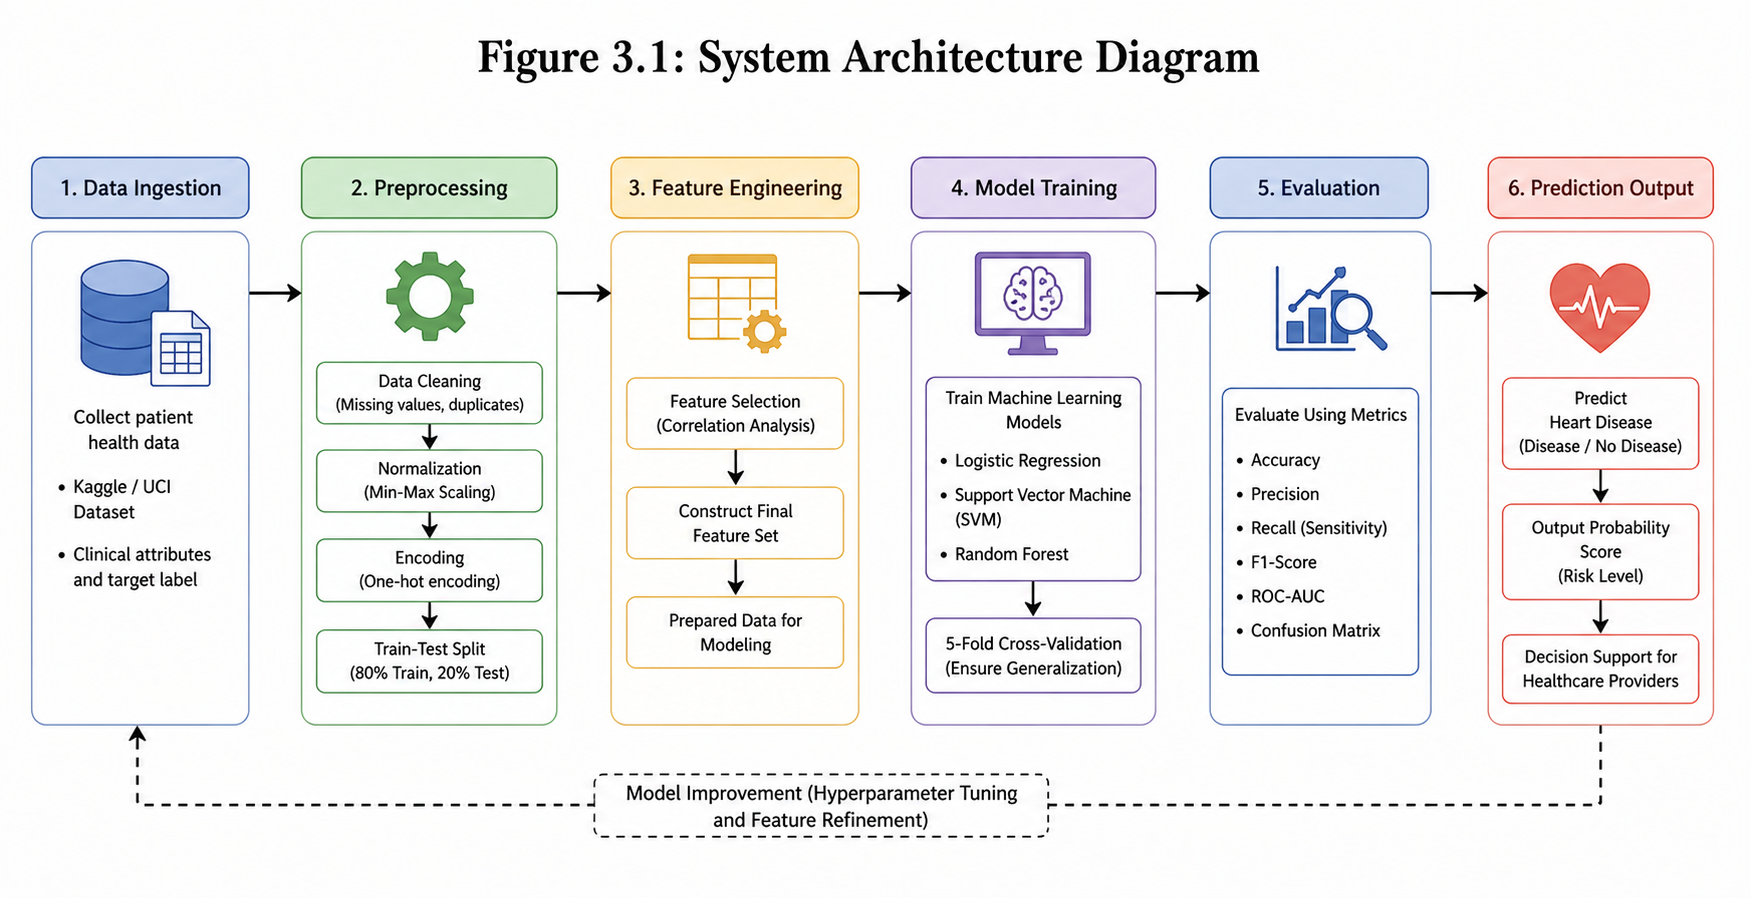
\includegraphics[width=\textwidth]{p 3.1.png}
  \caption{High-level system architecture of the proposed heart disease
           detection pipeline.}
  \label{fig:architecture}
\end{figure}

\begin{enumerate}
  \item \textbf{Data Ingestion Layer.} Imports structured clinical records from
    the combined UCI repository, covering Cleveland, Hungary, Switzerland, and
    Long Beach VA~\cite{uci_heart,detrano1989}.

  \item \textbf{Preprocessing Engine.} Imputes missing values, removes
    outliers, and applies Min-Max normalisation. Stratified splitting preserves
    the disease/no-disease class balance.

  \item \textbf{Feature Engineering.} Applies one-hot encoding for categorical
    variables and correlation-based feature selection to retain the strongest
    cardiac risk indicators.

  \item \textbf{Modelling Layer.} Trains Logistic Regression, SVM, and Random
    Forest~\cite{rf_heart2021} under stratified 5-fold
    cross-validation.

  \item \textbf{Evaluation \& Output Layer.} Generates class predictions and
    probability scores, enabling risk stratification and clinical referral.
\end{enumerate}

\begin{figure}[H]
  \centering
  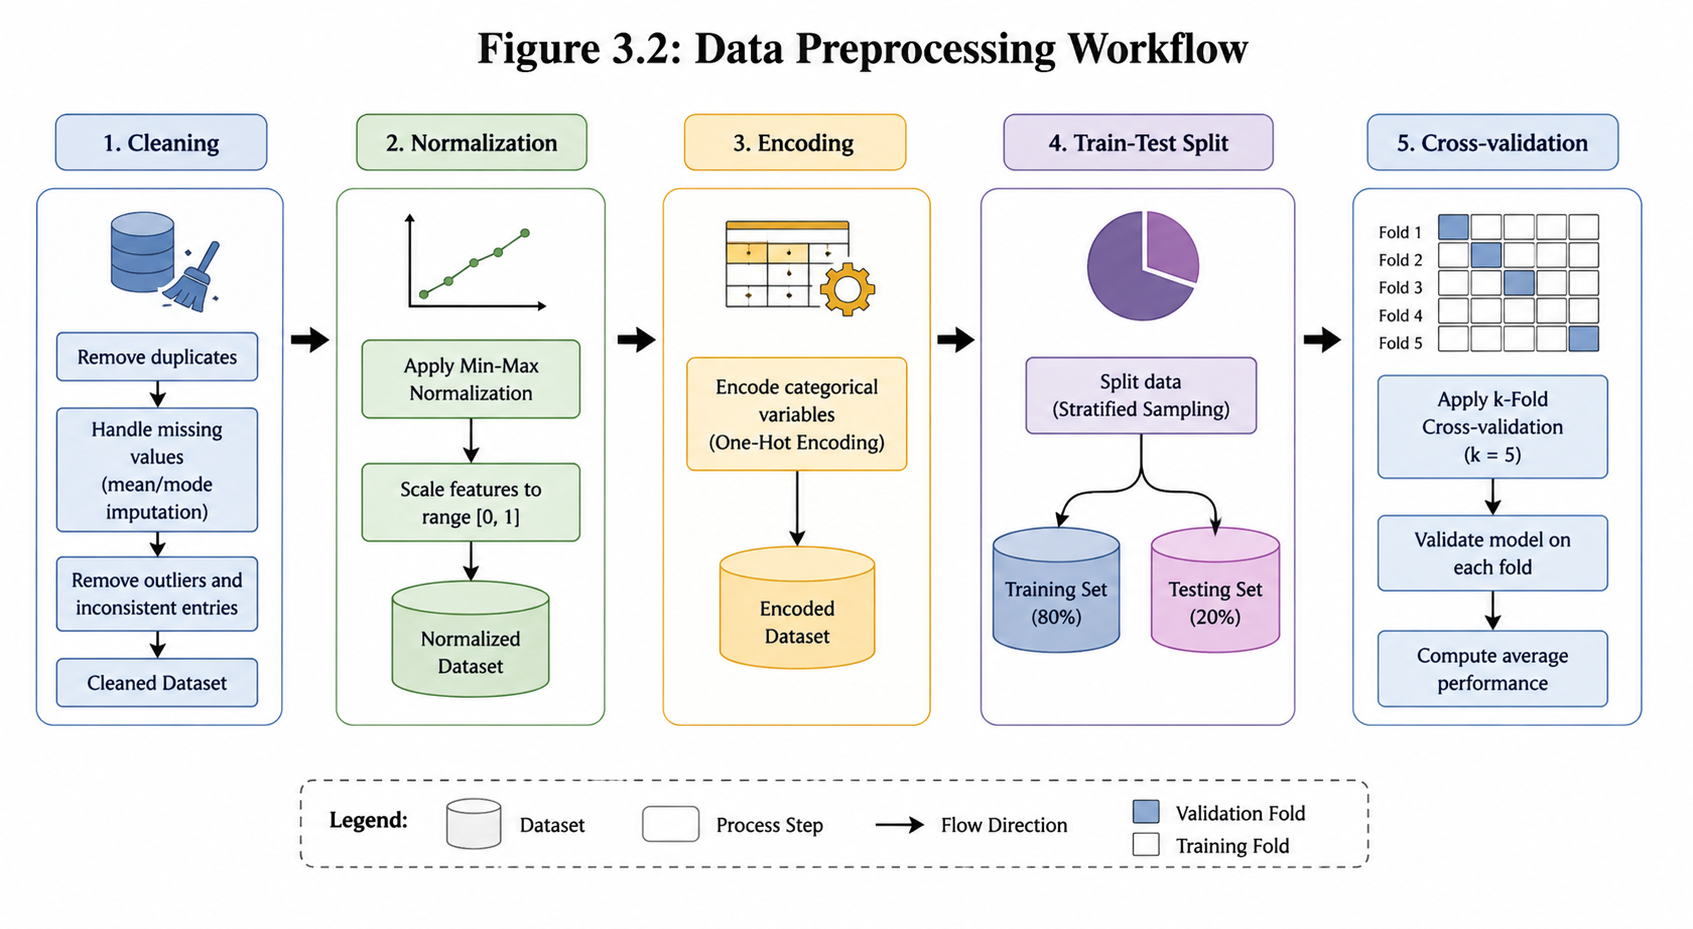
\includegraphics[width=\textwidth]{p 3.2.png}
  \caption{Detailed preprocessing and model-evaluation pipeline.}
  \label{fig:pipeline}
\end{figure}

\subsection{Tool Justification}

\textbf{Python \& Scikit-learn}~~are selected for their
efficiency with structured tabular medical data. Unlike deep learning
frameworks, Scikit-learn models require minimal compute, making them viable on
standard clinic hardware in underserved regions.

\textbf{Pandas \& NumPy}~~handle data loading, cleaning,
and numerical operations for the multi-source UCI dataset.

\textbf{Matplotlib \& Seaborn}~~generate ROC curves, confusion matrices, and
feature-importance plots so that model insights remain accessible to
non-specialist healthcare providers.

\subsection{Data Strategy}

\textbf{Dataset.}~The \textit{Combined Heart Disease Dataset} (UCI Machine
Learning Repository) merges records from Cleveland, Hungary, Switzerland, and
Long Beach VA into approximately \textbf{918 instances with 11 clinical
features}~\cite{uci_heart,detrano1989}. This addresses the small-sample
limitation identified in prior work~\cite{singh2024}.

\medskip
\textbf{Preprocessing pipeline:}
\begin{enumerate}
  \item Remove duplicate and structurally inconsistent rows.
  \item Impute missing values: mean for continuous features, mode for categorical.
  \item Apply Min-Max normalisation to scale every feature $x$ to $[0,1]$:
        $x' = (x - x_{\min})/(x_{\max} - x_{\min})$.
  \item One-hot-encode nominal categorical variables.
\end{enumerate}

\textbf{Splitting.}~An 80\,\%/20\,\% stratified train/test split is applied.
5-fold stratified cross-validation is used during training to reduce variance
in performance estimates.

\subsection{Evaluation Metrics}

All metrics are computed from the four entries of the binary confusion matrix:
true positives ($TP$), true negatives ($TN$), false positives ($FP$), and false
negatives ($FN$).

\subsubsection*{Accuracy}
The proportion of all samples correctly classified:
\begin{equation}
  \text{Accuracy} = \frac{TP + TN}{TP + TN + FP + FN}
  \label{eq:accuracy}
\end{equation}

\subsubsection*{Precision}
The fraction of positive predictions that are genuinely positive---measures
false-alarm rate:
\begin{equation}
  \text{Precision} = \frac{TP}{TP + FP}
  \label{eq:precision}
\end{equation}

\subsubsection*{Recall (Sensitivity)} \label{sec:recall}
The fraction of actual positive cases correctly identified---\textbf{the
primary metric} of this study, because missing a true heart disease case
($FN$) is clinically more harmful than a false alarm~\cite{rf_heart2021}.
Target: $\text{Recall} \geq 0.90$.
\begin{equation}
  \text{Recall} = \frac{TP}{TP + FN}
  \label{eq:recall}
\end{equation}

\subsubsection*{F1-Score}
The harmonic mean of Precision and Recall, which balances both concerns:
\begin{equation}
  F_1 = 2 \cdot \frac{\text{Precision} \times \text{Recall}}
                      {\text{Precision} + \text{Recall}}
  \label{eq:f1}
\end{equation}

\subsubsection*{ROC-AUC}
The Area Under the Receiver Operating Characteristic curve measures the
model's ability to discriminate between classes across all decision
thresholds~\cite{rf_heart2021}:
\begin{equation}
  \text{AUC} = \int_{0}^{1} \mathrm{TPR}(t)\,\mathrm{d}\,\mathrm{FPR}(t)
  \label{eq:auc}
\end{equation}
where $\mathrm{TPR}(t) = TP/(TP+FN)$ and $\mathrm{FPR}(t) = FP/(FP+TN)$ are
evaluated at threshold $t$. An AUC of 1.0 denotes perfect discrimination;
0.5 denotes random guessing.

\medskip
Table~\ref{tab:metric_summary} summarises the role and clinical significance
of each metric.

\begin{table}[H]
  \centering
  \caption{Summary of evaluation metrics and their clinical relevance.}
  \label{tab:metric_summary}
  \renewcommand{\arraystretch}{1.3}
  \begin{tabularx}{\textwidth}{@{} l l X @{}}
    \toprule
    \rowcolor{darknavy}
    \textcolor{white}{\textbf{Metric}} &
    \textcolor{white}{\textbf{Formula (ref.)}} &
    \textcolor{white}{\textbf{Clinical significance}} \\
    \midrule
    \rowcolor{lightgray}
    Accuracy          & Eq.~\eqref{eq:accuracy}    & Overall correctness across all patients. \\
    Precision         & Eq.~\eqref{eq:precision}   & Controls unnecessary follow-up for healthy patients. \\
    \rowcolor{lightgray}
    Recall            & Eq.~\eqref{eq:recall}      & \textbf{Primary.} Minimises missed diagnoses. \\
    F1-Score          & Eq.~\eqref{eq:f1}          & Balanced view when class sizes differ. \\
    \rowcolor{lightgray}
    ROC-AUC           & Eq.~\eqref{eq:auc}         & Threshold-independent discriminative power. \\
    \bottomrule
  \end{tabularx}
\end{table}

% ===========================================================
%  4. PROJECT MANAGEMENT & ETHICS
% ===========================================================
\section{Project Management \& Ethics}

\subsection{Project Timeline}

Figure~\ref{fig:gantt} illustrates the expected execution timeline for the
research project, spanning 13 weeks from initial data collection through final
testing and deployment preparation.

\begin{figure}[H]
  \centering
  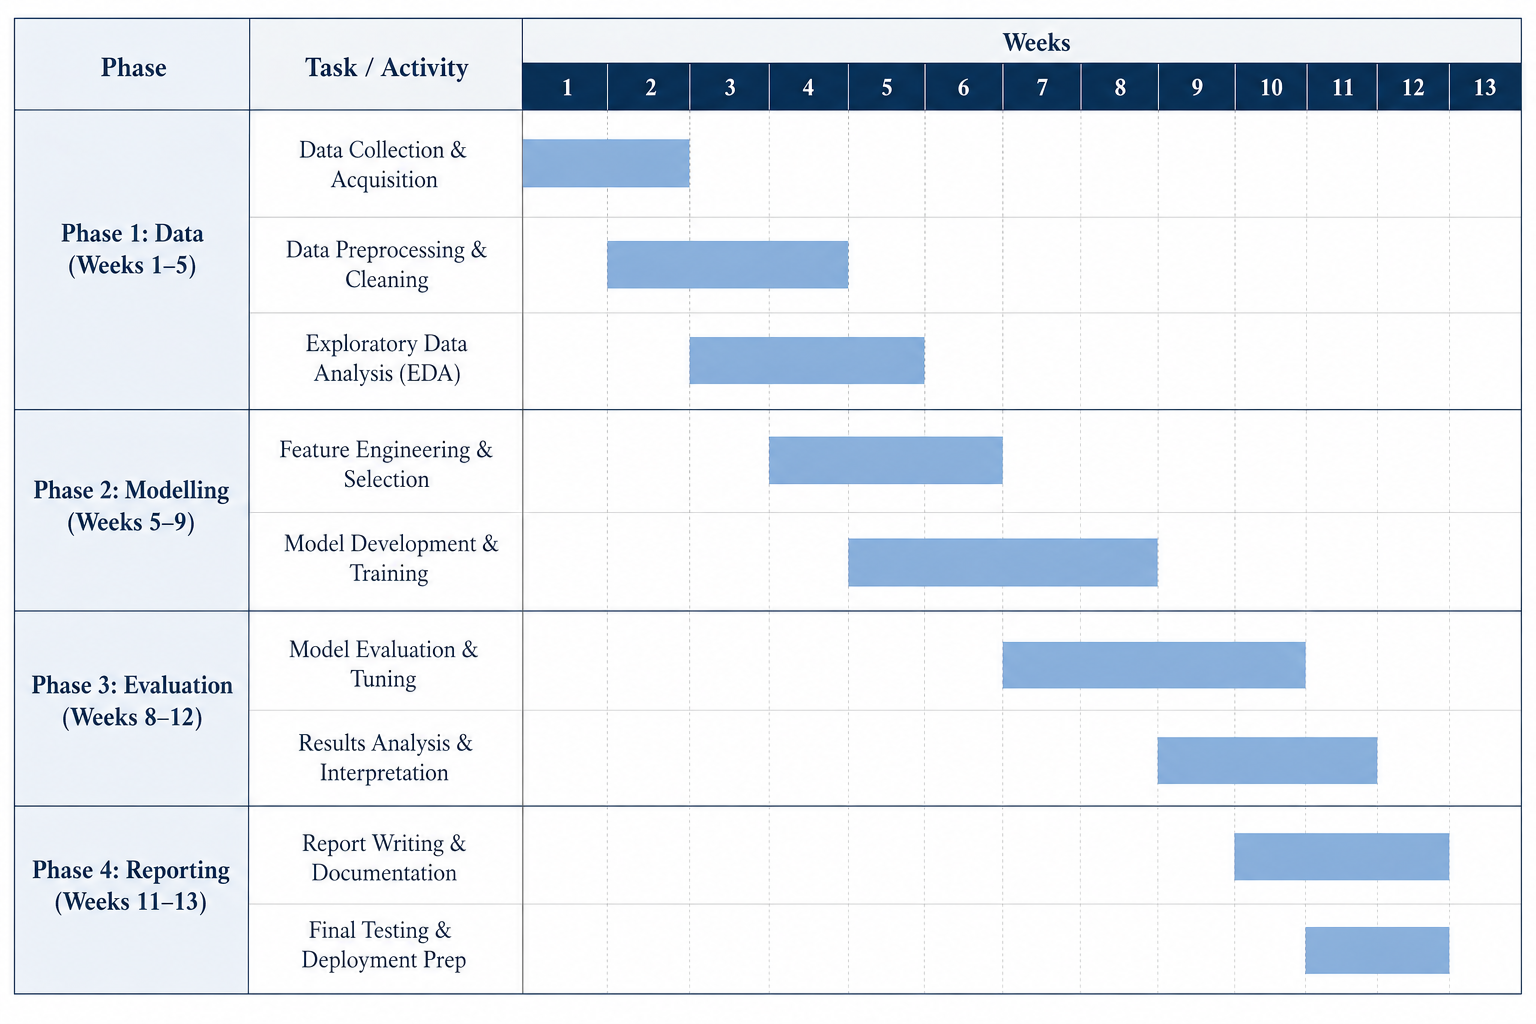
\includegraphics[width=0.97\textwidth]{gantt.png}
  \caption{Expected Project Execution Timeline (13 Weeks).}
  \label{fig:gantt}
\end{figure}

\subsection{Ethical Considerations}

\begin{itemize}
  \item \textbf{Data Privacy (GDPR).} The project uses only fully anonymised
    public datasets from the UCI Machine Learning
    Repository~\cite{uci_heart}. No personally identifiable information (PII)
    is processed, ensuring compliance with GDPR patient-confidentiality
    requirements.

  \item \textbf{Algorithmic Bias.} Stratified sampling during training and
    evaluation ensures that predictive accuracy is consistent across age groups
    and sexes, reducing the risk of discriminatory diagnostic recommendations.

  \item \textbf{Environmental Impact.} By selecting computationally efficient
    supervised models (Random Forest,
    SVM)~\cite{rf_heart2021} over deep learning architectures,
    the framework minimises energy consumption---a ``Green AI'' principle that
    also makes the system deployable on low-power hardware in underserved
    clinics.
\end{itemize}

% ===========================================================
%  BIBLIOGRAPHY
% ===========================================================
\newpage
\bibliographystyle{plainnat}
\bibliography{reference}
\addcontentsline{toc}{section}{References}

\end{document}